\documentclass[12pt,a4paper]{amsart}
% ukazi za delo s slovenscino -- izberi kodiranje, ki ti ustreza
\usepackage[slovene]{babel}
\usepackage[utf8]{inputenc}
\usepackage[T1]{fontenc}
\usepackage{multirow}
\usepackage{amsmath,amssymb,amsfonts}
\usepackage{url}
\usepackage[normalem]{ulem}
\usepackage[dvipsnames,usenames]{color}
\usepackage{csquotes}
\usepackage{caption}
\usepackage{lipsum}
\usepackage{hyperref}
\usepackage{tikz}
\usepackage{listings}
\usepackage{xcolor}
\usepackage{graphicx}
\usepackage{subcaption}


\lstset{
    breaklines=true,    
    breakatwhitespace=false,
    postbreak=\space,   
    tabsize=2,    
    basicstyle=\small\ttfamily\bfseries,
    commentstyle=\color{green!50!black},
    keywordstyle=\color{blue},
    numberstyle=\tiny\color{gray},
    numbers=left
}
\usetikzlibrary{graphs}
\usetikzlibrary{graphs.standard}

\makeatletter
\renewcommand\section{\@startsection{section}{1}%
  \z@{.5\linespacing\@plus.7\linespacing}{.5\linespacing}%
  {\normalfont\scshape\large\centering}}
\renewcommand\subsection{\@startsection{subsection}{2}%
  \z@{.5\linespacing\@plus.7\linespacing}{.5\linespacing}%
  {\normalfont\scshape}}
\renewcommand\subsubsection{\@startsection{subsubsection}{3}%
  \z@{.5\linespacing\@plus.7\linespacing}{-.5em}%
  {\normalfont\itshape}}
\makeatother

% ne spreminjaj podatkov, ki vplivajo na obliko strani
\textwidth 15cm
\textheight 24cm
\oddsidemargin.5cm
\evensidemargin.5cm
\topmargin-5mm
\addtolength{\footskip}{10pt}
\pagestyle{plain}
\overfullrule=15pt % oznaci predlogo vrstico


% ukazi za matematicna okolja
\theoremstyle{plain} % tekst napisan pokoncno
\newtheorem{definicija}{Definicija}[section]
\newtheorem{primer}[definicija]{Primer}
\newtheorem{definition}{Definicija}[section]

\renewcommand\endprimer{\hfill$\diamondsuit$}

% za stevilske mnozice uporabi naslednje simbole
\newcommand{\R}{\mathbb R}
\newcommand{\N}{\mathbb N}
\newcommand{\Z}{\mathbb Z}
\newcommand{\C}{\mathbb C}
\newcommand{\Q}{\mathbb Q}

% ukaz za slovarsko geslo
\newlength{\odstavek}
\setlength{\odstavek}{\parindent}
\newcommand{\geslo}[2]{\noindent\textbf{#1}\hspace*{3mm}\hangindent=\parindent\hangafter=1 #2}

% naslednje ukaze ustrezno popravi
\newcommand{\program}{Finančna matematika} % ime studijskega programa: Matematika/Finančna matematika
\newcommand{\imeavtorja}{Miha Jan, Sara Žužek} % ime avtorja
\newcommand{\imementorja}{doc. dr. Janoš Vidali} % akademski naziv in ime mentorja
\newcommand{\imesomentorja}{prof. dr. Riste Škrekovski}
\newcommand{\naslovdela}{Weak k-Metric Dimension}
\newcommand{\letnica}{2024} %letnica 


%%%%%%%%%%%%%%%%%%%%%%%%%%%%%%%%%%%%%%%%%%%%%%%%%%%%%%%%%%%%%%%%%%%%%%%%%%%%%%%%%%%%%%%%%%
\begin{document}

\thispagestyle{empty}
\noindent{\large
UNIVERZA V LJUBLJANI\\[1mm]
FAKULTETA ZA MATEMATIKO IN FIZIKO\\[5mm]
\program\ }
\vfill

\begin{center}{\large
\imeavtorja\\[2mm]
{\bf \naslovdela}\\[10mm]
Skupinski projekt\\[2mm]
Poročilo\\[1cm]
Mentorja: \imementorja, \\ \imesomentorja\\[2mm]}
\end{center}
\vfill

\noindent{\large
Ljubljana, januar \letnica}
\pagebreak

%%%%%%%%%%%%%%%%%%%%%%%%%%%%%%%%%%%%%%%%%%%%%%%%%%%%%%%%%%%%%%%%%
\section{Navodilo naloge}
Implement an ILP model for this invariant, and then write separate
small programs in Sage to answer each of following questions by exhaustive search.
\begin{enumerate}
    \item Find graphs for which $wdim_k(G) = \Delta(x, y)$ for a pair of vertices $x, y \in V(G)$ such that
    $d(x, y) \geq 3$.
    \item Determine $\kappa(G)$ and $wdim_k(G)$ for Cartesian products of cycles $G = C_a \square C_b$.
    \item  Determine the graphs G with $wdim_k(G) = dim_k(G)$ for various k with $k \leq \kappa(G)$.
\end{enumerate}
For small graphs, apply a systematic search; for larger ones, apply some stochastic search.
\bigskip
%%%%%%%%%%%%%%%%%%%%%%%%%%%%%%%%%%%%%%%%%%%%%%%%%%%%%%%%%%%%%%%%%
\section{Način reševanja problema}
Najina projektna naloga se navezuje na k-te šibke dimenzije grafov. Projekt sva razdelila na več manjših delov, od katerih vsak reši eno izmed podnalog. Natančnejši prgled najinega dela je opisan v nadaljevanju, tukaj pa je le kratek opis postopkov naijnega dela.

Najprej sva napisala ustrezen CLP, ki izračuna šibko k-to dimenzijo tega grafa. V nadaljevanju sva za vsako izmed podnalog napisala svojo funkcijo, ki je za izbran graf izračunala v navodilih podane karakteristike in funkcijo, ki je generirala željene grafe in testirala prej napisano kodo. 

V nadaljevanju sva napisala še kodo, ki sva jo testirala na večjih grafih in je temeljila na metahevrističnem algoritmu imenovanem simmulated annealing.

\bigskip
Najin cilj je bil, na podlagi testiranja oz. generiranja, ugotoviti, če za grafe, ki ustrezajo določenim 
pogojem veljajo kakšne posebne lastnosti. 
Za majhne vrednosti vozlišč sva se problema lotila s testiranjem na vseh grafih, 
za večje grafe pa sva kodo testirala le na naključnih grafih.

\bigskip
Za reševanje opisanega problema sva uporabila okolje Sage (SageMath) znotraj spletne platforme CoCalc. 
V nadaljevanju bova opisala in dodala kodo le od nekaterih funkcij, celotna koda s komentarji
se nahaja na GitHub repozitorju, prilagava tudi \href{https://github.com/mihajan/Weak-k-Metric-Dimension}{povezavo}.


\bigskip
%%%%%%%%%%%%%%%%%%%%%%%%%%%%%%%%%%%%%%%%%%%%%%%%%%%%%%%%%%%%%%%%%
\section{Definicije}
Za lažje razumevanje najinega problema, si najprej poglejmo par definicij, ki sva jih uporabljala v sklopu projektne naloge.
\begin{definition}
    Naj bo $S \subseteq V(G)$ in $a, b \in V(G)$. Definiramo $\Delta_S (a,b)$ kot vsoto razlik razdalj od $a$ in $b$ do vsakega vozlišča $S$. 
    Torej je $$\Delta_S (a,b) = \sum_{s \in S } |d(s,a) - d(s,b)|.$$
    Označimo $\Delta_{V(G)} (a,b) = \Delta (a,b)$.
\end{definition}

\begin{definition} 
    {\bf Šibka (vozliščna) k-metrična dimenzija} grafa $G$ $wdim_k(G)$, je kardinalnost/moč
    najmanjše množice vozlišč $S$ grafa $G$, tako da za vsak par vozlišč $x,y \in V(G)$ velja $\Delta_S (x,y) \geq k$.
\end{definition}

\begin{definition}
    Največja vrednost parametra $k,$ za katerega je šibka k-metrična dimenzija grafa G smiselno definirana označimo z $\kappa(G)$. 
\end{definition}

\begin{definition}
    {\bf K-metrična dimenzija} grafa $G$ $dim_k(G)$ je velikost najmanjše množice vozlišč $S$ grafa $G$, ki reši graf $G$ in ji rečemo k-rešljiva množica. 
    Za razliko od standardne metrične dimenzije ta zahteva, da vsak par vozlišč reši vsaj k vozlišč. K-metrična dimenzija se ujema z običajno dimenzijo, ko je $k = 1$.
\end{definition}
\bigskip


%%%%%%%%%%%%%%%%%%%%%%%%%%%%%%%%%%%%%%%%%%%%%%%%%%%%
\section{Majhni grafi}
Najprej sva se osredotočila na pisanje funkcije, ki s pomočjo ustreznega in učinkovitega CLP izračuna
k-to šibko dimnezijo. Funkcija sprejme graf G in število k, ter vrne vrednost šibke k-metrične dimenzije grafa
ob upoštevanju potrebnih pogojev.
\bigskip 
\begin{small}
    \begin{lstlisting}
    import itertools

    def CLP_weak_k_dim(g, k_value):
        p = MixedIntegerLinearProgram(maximization=False)
        x = p.new_variable(binary = True)
        p.set_objective(sum(x[v] for v in g))

        vertices = list(g.vertices())
        for va, vb in itertools.combinations(vertices, 2):
            expr = sum(abs(g.distance(va, vi) - g.distance(vb, vi)) * x[vi] for vi in g)
            p.add_constraint(expr >= k_value)

        sum_x = sum(x[vi] for vi in g)
        p.add_constraint(sum_x >= k_value)

        optimalna_resitev = p.solve()

        return optimalna_resitev
    \end{lstlisting}
\end{small}
\bigskip

Nato sva s pomočjo vgrajene metode \verb|distances_all_pairs| definirala funkcijo \verb|all_distances(graph)|, ki izračuna 
razdalje med vsemi pari vozlišč. 
Definirala sva še dve funkciji, ki jih bova potrebovala kasneje za reševanje najinih podnalog. 

Prva (\verb|delta(graph)|) izračuna $\Delta(x,y)$ za vse pare vozlišč in vrne izračunane vrednosti v slovarju,
druga (\verb|kappa(graph)|) pa izračuna vrednost $\kappa(G)$.

\begin{lstlisting}
    def delta(graph):
        dist = all_distances(graph)
        vertices = graph.vertices()
        delta_results = {}
        for x in vertices:
            for y in vertices:
                if x != y:
                    delta_xy = sum(abs(dist[s][x] - dist[s][y]) for s in vertices)
                    delta_results[(x, y)] = delta_xy
                else:
                    continue
        return delta_results
\end{lstlisting}

\begin{lstlisting}
    def kappa(graph):
        delta_results = delta(graph)
        min_delta = min(delta_results.values())
        return min_delta
\end{lstlisting}
\bigskip

%%%%%%%%%%%%%%%%%%%
\subsection{Prvi del naloge}
V prvem delu naloge sva morala poiskati grafe za katere velja, da je  $wdim_k(G) = \Delta(x, y)$, 
pri čemer je razdalja med dvema vozliščema $x$ in $y$ večja ali enaka 3. 
\bigskip

Najprej lahko opazimo, da zaheva za $dist(x,y) \geq 3$ pomeni, da mora naš graf imeti najmanj 4 vozlišča, da je ta zahteva izpolnjena. Nadalje lahko za taki vozlišči ugotovimo, da velja $\Delta(x,y) \geq 8,$ saj se njuni razdalji razlikujeta za vrednost 3 do vsakega izmed vozlišč $x$ in $y$ ter še za 1 do vsakega vmesnega vozlišča. Iz tega neposredno sledi, da bo iskana enakost lahko nastopila le na grafih z 8 ali več vozlišči. 

\bigskip

Definirala sva funkcijo 
\verb|ujemanje_1(graph)|, ki za izbrani graf poišče vse pare vozlišč, ki so med sabo oddaljeni za
3 ali več ter izračuna njihove $\Delta(x,y)$. Nato izračuna vse smislene šibke dimenzije za podani graf. Torej vse dimenzije od vključno 1. do $\kappa(g)$.
Funkcija nato vrne vrednost True, če je za podan graf našla ujemanje za katerokoli dimenzijo s poljubnim ustreznim $\Delta(x,y),$ sicer pa vrne False.

V nadaljevanju sva napisala funkcijo s pomočjo katere sva našla grafe, ki ustrezajo najinim pogojem. 
Napisana funkcija je za generiranje grafov uporabljala paket nauty geng, ki je  generiral vse povezane grafe, ki imajo najmanj m in največ n 
vozlišč (vrednosti m in n sva poljubno spreminjala). Problem, ki se je pojavil je ta, da je algoritem za veliko
število vozlišč prepočasen in ni sposoben pregledati vseh povezanih grafov, saj jih je preveč. Zato sva napisala 
drugo funkcijo, ki je pregledovala le naključne grafe, preostale pa je izpustila. 
\bigskip

%%%%%%%%%%%%%%%%%%%
\subsection{Drugi del naloge}
V tem delu naloge morava določiti $\kappa(G)$ in $wdim_k(G)$ za kartezične produkte ciklov $G = C_a \square C_b$.

Definirala sva funkcijo, ki sprejme dimenziji ciklov a in b in naredi njun kartezični produkt ter na njem izračuna željene vrednosti 
$\kappa(G)$ in $wdim_k(G)$ za vse k med 1 in $\kappa(G)$.

Napisala sva še nekja algoritmov s pomočjo katerih sva testirala željene parametre na takih grafih.
\bigskip

%%%%%%%%%%%%%%%%%%%
\subsection{Tretji del naloge}
Najprej sva definirala CLP, ki je podoben zgornjemu, le da namesto šibke k-te dimenzije izračuna k-to dimenzijo grafa.
Napisala sva funkciji 
\verb|kappa_navadna(graph)| in \verb|delta_navadna(graph)|, ki izračunata podobno kot prej predstavljeni funkciji, le da to naredita za navadno k-to dimenzijo grafov. 

Potem sva definirala funkcijo, ki za izbrani graf preveri, za katere dimenzije pride do ujemanj k-te in šibke k-te dimenzije grafa.
Ta funkcija vrne slovar, kjer so ključi slovarja vrednosti parametra k, za katere se dimenziji ujemata, vrednosti pa so enake pripadajoči k-ti oz. šibki k-ti dimenziji.
Napisala sva tudi algoritem, ki deluje podobno kot tisti pri prvem delu naloge, le da ta poleg grafa
izpiše še, katere k-te in k-te šibke dimenzije grafa se ujemajo.
Zaradi velikega števila ujemanj dimenzij sva se osredotočila na iskanje takih grafov, ki se ujemajo v vseh za njih izračunljivih dimenzijah.
Zato sva napisala tudi funkcijo, ki preveri ujemanja le za posebne primere grafov, kot so posplošeni Petersenovi grafi in hiperkocke.


%%%%%%%%%%%%%%%%%%%%%%%%%%%%%%%%%%%%%%%%%%%%%%%%%%%%%%%%%%%%%%%%%
\section{Ugotovitve}
\subsection{Prvi del naloge}
Najprej sva se še s testiranjem prepričala, da enakost za povezane grafe začne veljati šele pri grafih z vsaj 8 vozlišči, saj sva pregledala vse manjše grafe in nisva našla nobene enakosti.
Našla pa sva 8 grafov, ki imajo 8 vozlišč in ustrezajo danim pogojem. Opazila sva, da vsi ustrezni grafi vsebujejo
tudi cikle dolžine 3, kar pa se je pri večjih grafih izkazalo, da ne velja v splošnem. Vseh povezanih grafov z 8 vozlišči je 11.117, kar pomeni, da je vsak 1400 tak, 
ki ustreza najinim pogojem, oziroma $0,07 \%$ vseh grafov. Spodnja tabela prikazuje koliko je grafov na 8 vozliščih z določenim številom povezav. 
Vidimo da imajo vsi med 10-15 povezav, ter da je aritmetična sredina $11,75$, mediana pa 11.

\begin{table}[h]
    \begin{center}
      \begin{tabular}{l|c} % <-- Alignments: 1st column left, 2nd middle and 3rd right, with vertical lines in between
        \textbf{Število povezav} & \textbf{Število grafov} \\
        \hline
        10 & 2 \\
        11 & 3 \\
        12 & 1 \\
        14 & 1 \\
        15 & 1 \\
      \end{tabular}
    \end{center}
    \caption{Število povezav za grafe z 8 vozlišči}
    \label{tab:tabela1}
\end{table}

\bigskip
\begin{figure}[h]
    \centering
    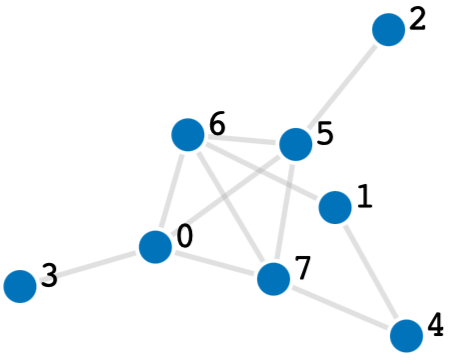
\includegraphics[width=0.25\textwidth]{slike/graf1.png}
    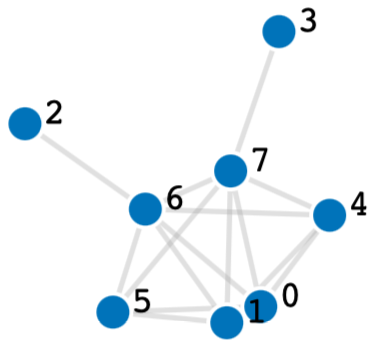
\includegraphics[width=0.25\textwidth]{slike/graf2.png}
    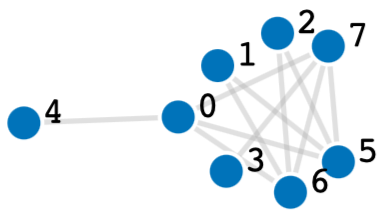
\includegraphics[width=0.25\textwidth]{slike/graf3.png}
    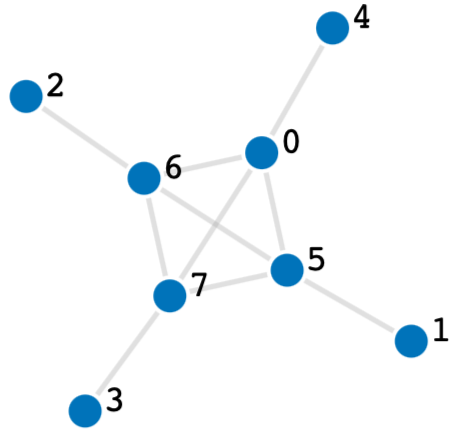
\includegraphics[width=0.25\textwidth]{slike/graf4.png}
    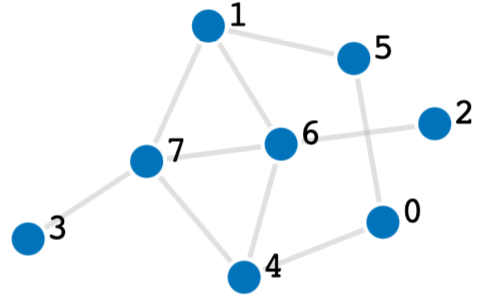
\includegraphics[width=0.25\textwidth]{slike/graf5.png}
    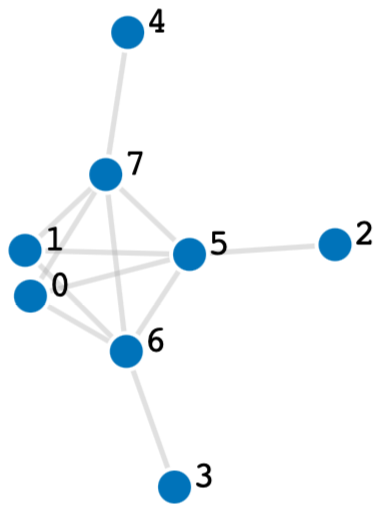
\includegraphics[width=0.25\textwidth]{slike/graf6.png}
    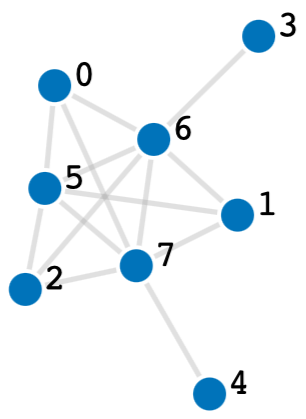
\includegraphics[width=0.2\textwidth]{slike/graf7.png}
    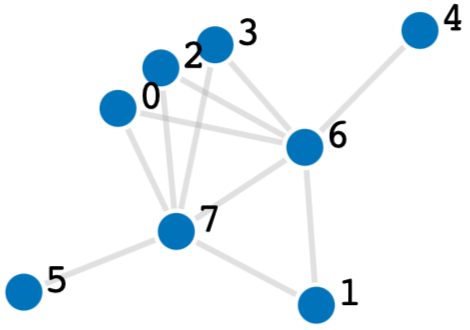
\includegraphics[width=0.25\textwidth]{slike/graf8.png}
    \caption{Vsi grafi z 8 vozlišči za katere velja enakost 1. podnaloge}
    \label{fig:slika1}
\end{figure}

Ujemanj na grafih z 9-mi vozlišči je mnogo več, celo tako veliko,
da program izpiše, da jih je preveč, da bi vse prikazal. Zato sva na tem mestu tudi začela osredotočati na delež ustreznih grafov glede na število vozlišč in ne na iskanje skupnih lastnosti, saj je bilo najdenih grafov preveč, da bi lahko našla njihove skupne lastnosti. 

Predvidevava, da se z naraščanjem števila vozlišč grafov število različnih $\Delta(x,y)$ za vozlišča, ki so oddaljena vsaj 3 veča zelo hitro.
Zato predvidevava, da je več možnosti, da pride do vsaj kakšnega ujemanja z $wdim_k(G)$ in posledično je vedno večji delež grafov na več vozliščih, ki ustrezajo zahtevani enakosti.

Z nadaljnim testiranjem sva poskusila preveritit to hipotezo in sva ugotovila, da pri grafih z 15 vozlišči pride do ujemanj že pri več kot $16 \%$ pregledanih grafov. Ko povečamo število vozlišč na 20 se tudi delež ujemanj poveča na $23 \%$.
Kodo sva testirala tudi za grafe med 20 in 25 vozlišč in ugotovila da je delež ujemanj na teh grafih znašal približno $25 \%$.
Ker pa je tako veliko ujemanj pa nisva uspela njati nobenega vzorca, 
ki bi za te grafe veljal. 
Torej z testiranjem sva nekako uspela potrditi, da z večanjem števila vozlišč, dobimo vedno več grafov, ki ustrezajo zahtevani enakosti, ne le po abosultni 
ampak tudi relativni spremembi. Na podlagi testov lahko trdiva, da zgornja lastnost ni prav redka za velike grafe. Spodaj si poglejmo še dva primera grafov z več vozlišči, ki ustrezata enakosti. 
\bigskip

\bigskip

\bigskip
\begin{figure}[h]
    \centering
    \begin{subfigure}{0.25\textwidth}
    \centering
    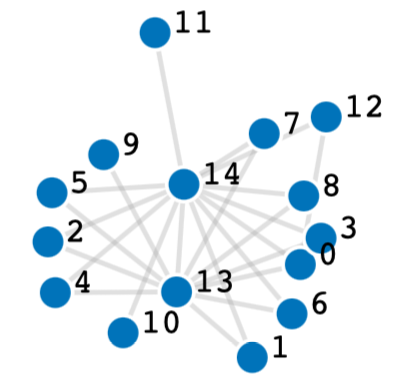
\includegraphics[width = \textwidth]{slike/graf15.png}
    \end{subfigure}
    \begin{subfigure}{0.25\textwidth}
    \centering
    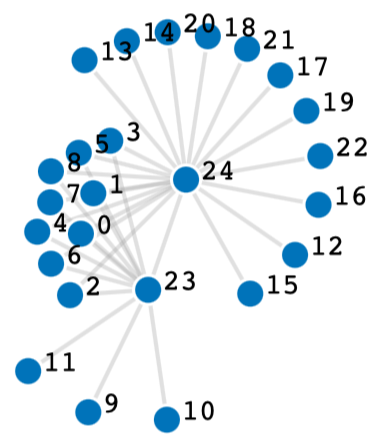
\includegraphics[width = \textwidth]{slike/graf25.png}
    \end{subfigure}
    \caption{Primer grafa s 15 in 25 vozlišči za katera velja enakost iz 1. podnaloge}
    \label{fig:slika2}
\end{figure}%


    
%%%%%%%%%%%%%%%%%%%
\subsection{Drugi del naloge}
Vzemimo cikel A s številom vozlišč $a$ in cikel B s številom vozlišč $b$, njun kartezični produkt G ima število vozlišč $a \cdot b$. 
Na podlagi testiranja do velikosti ciklov dimenzij $15 \times 15 $ sva ugotovila, da za vse pregledane grafe velja formula za $\kappa(G)$ glede na to ali imata cikla A in B liho oziroma sodo število vozlišč. 

Če imata oba cikla sodo število vozlišč, velja: $\kappa(G) = a \cdot b$.

Če imata oba liho število vozlišč, velja: $\kappa(G) = a \cdot b - max(a,b)$.

Če ima en liho in en sodo število vozlišč, pa velja: $\kappa(G) = a \cdot b - sodo(a,b)$.

Medtem, ko je $wdim_k(G)$, če za $k$ vzamemo $\kappa(G)$ kar enaka $a \cdot b$.


\bigskip
%%%%%%%%%%%%%%%%%%%
\subsection{Tretji del naloge}
Pri povezanih grafih, generiranih z nauty geng, število ujemanj s številom vozlišč močno narašča. 
Vemo, da že po definiciji velja ujemanje za $k = 1$, zato sva želela poiskati grafe, ki se ujemajo za različne k.

Tako imamo za grafe s 4 vozlišči, 3 grafe, za katere velja $wdim_k(G) = dim_k(G)$, kjer je poleg ujemanja za $k = 1$, 
ujemanje tudi pri $k = 2$.

Medtem, ko je takih grafov, ki se ujemajo za vsaj dva k 10 s petimi vozlišči in 54 s šestimi vozlišči. 

\bigskip

Spodaj so prikazane slike vseh treh grafov s štirimi vozlišči, ki imajo vsaj dve ujemanji.

\bigskip
\begin{figure}[h]
    \centering
    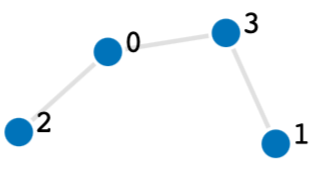
\includegraphics[width=0.22\textwidth]{slike/naloga3_12.png}
    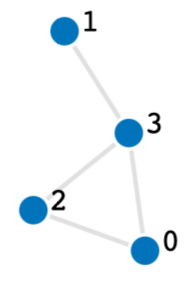
\includegraphics[width=0.17\textwidth]{slike/naloga3_23.png}
    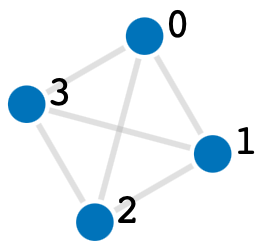
\includegraphics[width=0.17\textwidth]{slike/naloga3_34.png}
    \caption{Grafi, ki se ujemajo za $wdim_k(G)=dim_k(G)$ za $k = 1,2$}
    \label{fig:slika1}
\end{figure}

\bigskip

Na splošnih povezanih grafih sva hitro ugotovila, da obstaja zelo veliko grafov, ki se ujamajo vsaj v nekaj dimenzijah in nimajo skupnih lastnosti. Zato sva se osredotočila na nekaj značilnih skupin grafov in iskala grafe, ki se ujemajo v čim več dimenzijah.

Najprej sva pogledala poseben primer grafov in sicer cikle.
Naj bo $n$ število vozlišč cikla, ugotovila sva, da se lihi cikli ujemajo za vse $k$ od $1$ do $n - 1$ kar je tudi maksikmalna vrednost $k$ za katere se da izračunati dimenzijo cikla.
Sodi cikli pa se ujemajo le za $k = 1$. 

Posebej sva testirala tudi grafe, ki so kartezični produkti ciklov in ugotovila zanimivost, ki velja za produkte naslednjih dimenzij. Če imamo cikel A dolžine 3, cikel B 
pa je dolžine 6 ali več.
Velja, da se kartezični produkti oblike 3 x b, kjer je b sodo število, ujemajo za vse k, kjer je
$k = 1, 2, ... \kappa(G)$.
Za kartezične produkte 3 x b, kjer je b liho število pa je ujemanje enako kot za sode z izjemo 3 in 4.

\bigskip
Ob testiranju sva ugotovila, da se Petersenov graf ujema v vseh 6 dimenzijah. Zato sva napisala funkcijo, ki je testirala ujemanja za posplošene Peteresenove grafe (angl. Generalized Petersen graphs). Ugotovila sva, da se nobeden od teh grafov ne ujema v vseh dimenzijah tako kot navaden Petersenov, vendar za grafe kjer je $k=2$ in $n$ sodo število pride do ujemanja v zelo veliko dimenzijah. Tako se na primer GeneralizedPetersen(16,2) ujema v 10 dimenzijah, GeneralizedPetersen(18,2) pa v kar 11 dimenzijah. Če postavimo $k=1$ pa se za poljuben $n$ grafi ujemajo le v 1. dimenziji.  

\begin{table}[h]
    \centering
    \begin{tabular}{|c|c|}
        \hline
        k & vrednost \\
        \hline
        1 & 3.0 \\
        2 & 4.0 \\
        3 & 7.0 \\
        4 & 8.0 \\
        5 & 9.0 \\
        6 & 10.0 \\
        \hline
    \end{tabular}
    \caption{Dimenzije in ujemanja za Petersenov graf}
    \label{tab:python_output}
\end{table}

\begin{table}[h]
    \centering
    \begin{tabular}{|c|c|}
        \hline
        k & vrednost \\
        \hline
        1 & 3.0 \\
        2 & 4.0 \\
        3 & 5.0 \\
        9 & 13.0 \\
        18 & 26.0 \\
        19 & 27.0 \\
        20 & 29.0 \\
        21 & 31.0 \\
        22 & 33.0 \\
        23 & 35.0 \\
        24 & 36.0 \\
        \hline
    \end{tabular}
    \caption{Ujemanja za GeneralizedPetersen(18,2).}
    \label{tab:ujemanja_gp}
\end{table}

\begin{figure}[h]
    \centering
    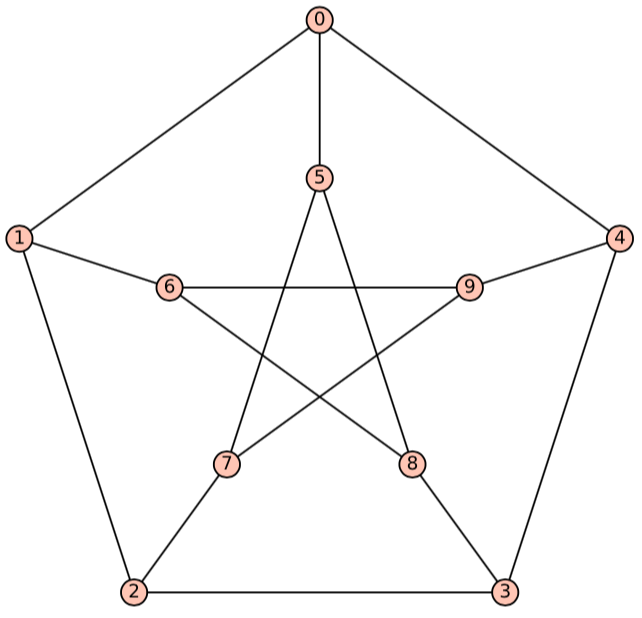
\includegraphics[width=0.35\textwidth]{slike/petersen.png}
    \caption{Klasičen Petersenov graf}
    \label{fig:slika1}
\end{figure}


%%%%%%%%%%%%%%%%%%%%%%%%%%%%%%%%%%%%%%%%%%%%%%%%%%%%%
\section{Simulated annealing}
Metodo simulated annealing sva dodala kot alternativo za velike grafe, saj najde približek rešitve precej hitreje kot prek računanja z CLP.

Napisani algoritem deluje tako, da sprejme graf, število k in poljubno množico vozlišč, ki jih določimo, da so v začetni množici $S$ ter specifične parametre za iskanje. Algoritem potem postopoma z uporabo verjetnosti prilagaja množico $S$ in poskuša poiskati najmanjšo tako množico vozlišč $S,$ ki zadošča pogojem iz definicike šibke k-te dimenzije.

Opazila sva, da je hitrost in natančnost tega algoritma zelo odvisna od tega kaj na prvem koraku vzamemo za začetno mnoćico $S$. Na primer če iščemo neko dimenzijo grafa za katero vemo, da bo zelo velika je priporočljivo vzeti za $S$ kar celotno množico vozlišč danega grafa.

Ob testiranju sva ugotovila, da kljub temu da je ta algoritem precej hitrejši od CLP-ja pa njegova hitrost na danih podnaloga ne odtehta njegove nenatančnosti, saj najde le približek za šibko dimenzijo ne pa njene točne vrednosti.

Torej uporabo tega algoritma bi priporočila le v primeru, ko nas zanima približna šibka k-ta dimenzija grafa, ne pa njegova točna dimenzija. 

\bigskip

%%%%%%%%%%%%%%%%%%%%%%%%%%%%%%%%%%%%%%%%%%%%%%%%%%%%%
\bigskip
Za pomoč pri nalogi sva uporabila spodnjo literaturo.
\begin{thebibliography}{99}
    \bibitem{peterin2023resolving}
    I. Peterin, J. Sedlar, R. Škrekovski, I. G. Yero,
    \emph{Resolving vertices of graphs with differences},
    (2023) arXiv preprint arXiv:2309.00922.
    \end{thebibliography}

\end{document}